% !TeX program = pdflatex
% !TeX spellcheck = en_US
% !TeX encoding = UTF-8

% update
% v.1.2 - 2018-10-15
% - Felix: use Bibtex instead of Biblatex
% v1.10 - 2017-05-30
% - Erik: Refactor the file structure of the front pages
% - Erik: Fix double bibliography entry
% v1.9 - 2017-02-03
% - Dirk: fixed warning: Underfull \hbox (badness 10000) in paragraph main.tex
% - Dirk: fixed warning: "Data encoding is UTF8" -> style.tex 0.1.8
% v1.8 - 2017-02-02
% - Dirk: replaced titlesec package by KOMA-script commands.-> style.tex v0.1.7
% v1.7 - 2014-11-18
% - bib fixes: now using biber instead of bibtex (thanks felix)
% - compile now with pdflatex -> biber -> pdflatex
% v1.6 - 2013-05-13
% - bibliography headers fixed - thanx lorenz lehmann
% - high quality titlepage - thanx thomas graf
% - removed separation of online and offline references -> style 1.4a
% v1.5 - 2013-01-16

\documentclass[twoside,11pt,titlepage,a4paper,english,bibliography=totocnumbered,listof=numbered]{scrbook}
% Copyright 2017 Sergei Tikhomirov, MIT License
% https://github.com/s-tikhomirov/solidity-latex-highlighting/

\usepackage{listings, xcolor}

\definecolor{verylightgray}{rgb}{.97,.97,.97}

\lstdefinelanguage{Solidity}{
	keywords=[1]{anonymous, assembly, assert, balance, break, call, callcode, case, catch, class, constant, continue, contract, debugger, default, delegatecall, delete, do, else, emit, event, export, external, false, finally, for, function, gas, if, implements, import, in, indexed, instanceof, interface, internal, is, length, library, log0, log1, log2, log3, log4, memory, modifier, new, payable, pragma, private, protected, public, pure, push, require, return, returns, revert, selfdestruct, send, storage, struct, suicide, super, switch, then, this, throw, transfer, true, try, typeof, using, value, view, while, with, addmod, ecrecover, keccak256, mulmod, ripemd160, sha256, sha3}, % generic keywords including crypto operations
	keywordstyle=[1]\color{blue}\bfseries,
	keywords=[2]{address, bool, byte, bytes, bytes1, bytes2, bytes3, bytes4, bytes5, bytes6, bytes7, bytes8, bytes9, bytes10, bytes11, bytes12, bytes13, bytes14, bytes15, bytes16, bytes17, bytes18, bytes19, bytes20, bytes21, bytes22, bytes23, bytes24, bytes25, bytes26, bytes27, bytes28, bytes29, bytes30, bytes31, bytes32, enum, int, int8, int16, int24, int32, int40, int48, int56, int64, int72, int80, int88, int96, int104, int112, int120, int128, int136, int144, int152, int160, int168, int176, int184, int192, int200, int208, int216, int224, int232, int240, int248, int256, mapping, string, uint, uint8, uint16, uint24, uint32, uint40, uint48, uint56, uint64, uint72, uint80, uint88, uint96, uint104, uint112, uint120, uint128, uint136, uint144, uint152, uint160, uint168, uint176, uint184, uint192, uint200, uint208, uint216, uint224, uint232, uint240, uint248, uint256, var, void, ether, finney, szabo, wei, days, hours, minutes, seconds, weeks, years},	% types; money and time units
	keywordstyle=[2]\color{teal}\bfseries,
	keywords=[3]{block, blockhash, coinbase, difficulty, gaslimit, number, timestamp, msg, data, gas, sender, sig, value, now, tx, gasprice, origin},	% environment variables
	keywordstyle=[3]\color{violet}\bfseries,
	identifierstyle=\color{black},
	sensitive=false,
	comment=[l]{//},
	morecomment=[s]{/*}{*/},
	commentstyle=\color{gray}\ttfamily,
	stringstyle=\color{red}\ttfamily,
	morestring=[b]',
	morestring=[b]"
}

\lstset{
	language=Solidity,
	backgroundcolor=\color{verylightgray},
	extendedchars=true,
	basicstyle=\footnotesize\ttfamily,
	showstringspaces=false,
	showspaces=false,
	numbers=left,
	numberstyle=\footnotesize,
	numbersep=9pt,
	tabsize=2,
	breaklines=true,
	showtabs=false,
	captionpos=b
}

%
% Template Style
% =========================================================================
% = SNET THESIS TEMPLATE STYLE
% =========================================================================

% http://www.snet.tu-berlin.de
% ------------------------
% Adapted version from http://hci.rwth-aachen.de/karrer_thesistemplate (Thorsten Karrer)
% Further adaptions for http://www.elearn.rwth-aachen.de (Sascha Hoellger)
% Further adaptions for SNET @ TU Berlin by Sebastian Göndör (sebastian.goendoer@tu-berlin.de)


% =========================================================================
% = CHANGELOG
% =========================================================================
% [0.1.9]
% - Fixed styling for chapters and toc using Komascript
% - Remove double bibliography TOC entry
%
% [0.1.8]
% - fixed "warning UFT8 is used". biblatex requires ascii encoding; by Dirk
%
% [0.1.7]
% replaced "Titelsec" commands (and whole package) by appropriate KOMA-Script commands; by Dirk
%
% [0.1.6]
% replaced deprecated \rm commands with \rmfamily commands; by Dirk
%
% [0.1.4b]
% backend=biber added in line 139
%
% [0.1.4a]
% title page: image logo sizes and margins adjusted to printable area
% removed separation of online and offline references
%
% [0.1.3]
% wider text body
% added "school" to the titlepage
% paragraph indents
% correctly placed footnote graphics
%
% [0.1.2]
% new titlepage
% some minor fixes
%
% [0.1.1]
% changed titlepage logo
% added listoffigures and listoftables
% excluded abstract from toc
% no (roman) numbering for frontmatter
%
% [0.1]
% adapted version 0.991b from sascha hoellger @ rwth aachen


% =========================================================================
% = MISC
% =========================================================================

\usepackage{a4wide}					%
\usepackage{verbatim}				%
\usepackage[toc,page]{appendix}			%
\usepackage[withpage]{acronym}			%
\usepackage{amsthm}				% Definitions


% =========================================================================
% = COLORS
% =========================================================================

\usepackage{xcolor}					% Colors
\definecolor{LightBlue}{rgb}{0.55,0.55,1}
\definecolor{DarkBlue}{rgb}{0.2,0.2,0.5}
\definecolor{DarkRed}{rgb}{0.71,0.12,0.07}

% =========================================================================
% = PAGE LAYOUT
% =========================================================================

\usepackage{geometry}
\geometry{inner=3cm, outer=2cm, bottom=4cm}

\newcommand{\setwidesite}				% changes the geometry to have less margin
{
	\fancyhfoffset[LE,RO]{0cm}
	\fancyheadoffset[LO,RE]{0cm}
	\fancyfootoffset[RE]{2cm}
	\newgeometry{inner=2cm, outer=2cm, bottom=4cm}
}

\usepackage{style/noindent}				%do not indent at new paragraphs but add a vertical offset

\setlength{\parindent}{4mm}
\setlength{\parskip}{1.5mm }


% =========================================================================
% = TYPESETTING
% =========================================================================

\usepackage[hyphens]{url}				% url
\usepackage{hyphenat}				% hyphenation. use \hyphenation{}

\righthyphenmin=5
\lefthyphenmin=5


% =========================================================================
% = TABLE OF CONTENTS
% =========================================================================

\setcounter{secnumdepth}{4}
\setcounter{tocdepth}{3}

\addtokomafont{disposition}{\rmfamily}


% =========================================================================
% = FONTS
% =========================================================================

\usepackage{mathpazo}
\usepackage[scaled=.95]{helvet}
\usepackage{courier}


% =========================================================================
% = SYMBOLS
% =========================================================================

%\usepackage{gensymb}
\usepackage{textcomp} 				% for \textmu (non-italic $\mu$)
\makeatletter						% this makes "@" a regular letter


% =========================================================================
% = TABLES
% =========================================================================

\usepackage{tabularx}
\usepackage{booktabs}
\usepackage{multirow}
\usepackage{longtable}				% tables spanning over more than one page

%%\setlength{\fboxsep}{0mm}			% spacing between \fbox border and content

\usepackage{amsmath}				% math fonts
\usepackage{amssymb}				% math symbols
\usepackage{setspace}				% line spacing


% =========================================================================
% = BIBILOGRAPHY
% =========================================================================

% 2018-10-16 - changed to use Bibtex instead

%\usepackage[style=numeric,natbib=true,backend=biber]{biblatex}

% apparently no effect?
%\renewcommand{\bibsetup}{
%	\markboth{
%		\MakeUppercase{Bibliography}
%	}{}
%}

%\ifdefined\bibheadingonline
%  \defbibheading{online}{\section*{\bibheadingonline}}
%\else
%  \defbibheading{online}{\section*{Online References}}
%\fi
%\ifdefined\bibheadingoffline
%  \defbibheading{offline}{\section*{\bibheadingoffline}}
%\else
%  \defbibheading{offline}{\section*{Printed References}}
%\fi
%
%\defbibfilter{online}{%
%  \( \type{online} \)}
%
%\defbibfilter{offline}{%
%  \( \not \type{online} \)}
%
%\bibliography{Bibliography}


% =========================================================================
% = LANGUAGE & ENCODING
% =========================================================================

\usepackage[english]{babel}				% \usepackage[ngerman]{babel}

\selectlanguage{english}				% \selectlanguage{ngerman}

\usepackage[T1]{fontenc}
\usepackage[utf8]{inputenc}				% can use native umlauts

% \usepackage[babel,german=quotes]{csquotes}	% provides \enquote{Blupp} => "`Blupp"'
\usepackage[babel,english=american]{csquotes}	% provides \enquote{Blupp} => "`Blupp"'

%\SetCiteCommand{\parencite}			% Changed for biblatex

\usepackage{units}					% unified way of setting values with units

\usepackage{appendix}


% =========================================================================
% = CODE LISTINGS
% =========================================================================

\usepackage{listings}

% Listings Styles from Max

\definecolor{violet}{cmyk}{0.45,0.97,0.27,0.21}
\definecolor{lstblue}{cmyk}{1,0.80,0,0}
\definecolor{lstgreen}{cmyk}{0.71,0.21,0.65,0.22}
\definecolor{bluegrey}{cmyk}{0.56,0.24,0.11,0.05}
\definecolor{javadoc}{cmyk}{0.88,0.59,0,0}
\definecolor{lstgrey}{cmyk}{0.55,0.44,0.42,0.32}

\lstdefinelanguage{SQL}{
     keywords={},
     keywordstyle=\color{bluegrey}\bfseries,
     morekeywords=[2]{CREATE,TABLE,IF,NOT,EXISTS,NULL,SET,DEFAULT,PRIMARY,KEY,COLLATE,CHARACTER,AUTO_INCREMENT,ENGINE,CHARSET},
     keywordstyle={[2]\color{violet}\bfseries},
     otherkeywords={int,varchar,double,text,tinyint},
     sensitive=false,
     morecomment=[l][\color{lstgreen}]{//},
     morecomment=[s][\color{lstgreen}]{/*}{*/},
     morecomment=[s][\color{javadoc}]{/**}{*/},
     morestring=[b]',
     morestring=[b]"
  }
\lstdefinelanguage{PHP}{
     keywords={},
     keywordstyle=\color{bluegrey}\bfseries,
     morekeywords=[2]{static,function,if,return,pow,sin,cos,asin,min,sqrt,int},
     keywordstyle={[2]\color{violet}\bfseries},
     otherkeywords={@param, @returns, @author, @type, @link, @see},
     sensitive=false,
     morecomment=[l][\color{lstgreen}]{//},
     morecomment=[s][\color{lstgreen}]{/*}{*/},
     morecomment=[s][\color{javadoc}]{/**}{*/},
     morestring=[b]',
     morestring=[b]"
  }
\lstdefinelanguage{JavaScript}{
     keywords={},
     keywordstyle=\color{bluegrey}\bfseries,
     morekeywords=[2]{attributes, class, classend, do, empty, endif, endwhile, fail, function, functionend, if, implements, in, inherit, inout, not, of, operations, out, return, set, then, types, while, use},
     keywordstyle={[2]\color{violet}\bfseries},
     otherkeywords={@param, @returns, @author, @type, @link, @see},
     sensitive=false,
     morecomment=[l][\color{lstgreen}]{//},
     morecomment=[s][\color{lstgreen}]{/*}{*/},
     morecomment=[s][\color{javadoc}]{/**}{*/},
     morestring=[b]',
     morestring=[b]"
  }
\lstdefinelanguage{Java}{
     keywords={},
     keywordstyle=\color{bluegrey}\bfseries,
     morekeywords=[2]{abstract,boolean,break,byte,case,catch,char,class,
      const,continue,default,do,double,else,extends,false,final,
      finally,float,for,goto,if,implements,import,instanceof,int,
      interface,label,long,native,new,null,package,private,protected,
      public,return,short,static,super,switch,synchronized,this,throw,
      throws,transient,true,try,void,volatile,while},
     keywordstyle={[2]\color{violet}\bfseries},
     morekeywords=[3]{@SuppressWarnings, @Capability, @Override},
     keywordstyle={[3]\color{lstgrey}},
     otherkeywords={@param, @return, @returns, @author, @link, @see},
     sensitive,
     morecomment=[l]//,
     morecomment=[s]{/*}{*/},
     morecomment=[s][\color{javadoc}]{/**}{*/},
     morestring=[b]",
     morestring=[b]',
  }[keywords,comments,strings]

% some listings styles from Gregor Aisch
% http://vis4.net/blog/2009/09/noch-mehr-sprach-definitionen-fuer-latex-listings/

\lstdefinelanguage{HTML5} {morekeywords={a, abbr, address, area, article, aside, audio, b, base, bb, bdo, blockquote,  body, br, button, canvas, caption, cite, code, col, colgroup, command, datagrid, datalist, dd, del, details, dialog, dfn, div, dl, dt, em, embed, eventsource, fieldset, figure, footer,  form,  h1, h2,  h3,  h4, h5,  h6,  head,  header,  hr, html,  i, iframe,  img,  input,  ins, kbd,  label,  legend,  li,  link,  mark,  map,  menu,  meta,  meter,  nav,  noscript,  object,  ol,  optgroup,  option,  output,  p,  param,  pre,  progress,  q,  ruby,  rp,  rt,  samp,  script,  section,  select,  small,  source,  span,  strong,  style,  sub,  sup,  table,  tbody,  td,  textarea,  tfoot,  th,  thead,  time,  title,  tr,  ul,  var,  video},
sensitive=false, morecomment=[s]{<!--}{-->}, morestring=[b]", morestring=[d]'}

\lstdefinelanguage{CSS} {morekeywords={azimuth,  background-attachment,  background-color,  background-image,  background-position,  background-repeat,  background,  border-collapse,  border-color,  border-spacing,  border-style,  border-top, border-right, border-bottom, border-left,  border-top-color, border-right-color, border-bottom-color, border-left-color,  border-top-style, border-right-style, border-bottom-style, border-left-style,  border-top-width, border-right-width, border-bottom-width, border-left-width,  border-width,  border,  bottom,  caption-side,  clear,  clip,  color,  content,  counter-increment,  counter-reset,  cue-after,  cue-before,  cue,  cursor,  direction,  display,  elevation,  empty-cells,  float,  font-family,  font-size,  font-style,  font-variant,  font-weight,  font,  height,  left,  letter-spacing,  line-height,  list-style-image,  list-style-position,  list-style-type,  list-style,  margin-right, margin-left,  margin-top, margin-bottom,  margin,  max-height,  max-width,  min-height,  min-width,  orphans,  outline-color,  outline-style,  outline-width,  outline,  overflow,  padding-top, padding-right, padding-bottom, padding-left,  padding,  page-break-after,  page-break-before,  page-break-inside,  pause-after,  pause-before,  pause,  pitch-range,  pitch,  play-during,  position,  quotes,  richness,  right,  speak-header,  speak-numeral,  speak-punctuation,  speak,  speech-rate,  stress,  table-layout,  text-align,  text-decoration,  text-indent,  text-transform,  top,  unicode-bidi,  vertical-align,  visibility,  voice-family,  volume,  white-space,  widows,  width,  word-spacing,  z-index},
sensitive=false, morecomment=[s]{/*}{*/}, morestring=[b]", morestring=[d]'}

\lstdefinelanguage{JavaFX} {morekeywords={abstract, after, and, as, assert, at, attribute, before, bind, bound, break, catch, class, continue, def, delete, else, exclusive, extends, false, finally, first, for, from, function, if, import, indexof, in, init, insert, instanceof, into, inverse, last, lazy, mixin, mod, new, not, null, on, or, override, package, postinit, private, protected, public-init, public, public-read, replace, return, reverse, sizeof, static, step, super, then, this, throw, trigger, true, try, tween, typeof, var, where, while, with },
sensitive=false, morecomment=[l]{//}, morecomment=[s]{/*}{*/}, morestring=[b]", morestring=[d]'}

\lstdefinelanguage{MXML} {morekeywords={mx:Accordion, mx:Box, mx:Canvas, mx:ControlBar, mx:DividedBox, mx:Form, mx:FormHeading, mx:FormItem, mx:Grid, mx:GridItem, mx:GridRow, mx:HBox, mx:HDividedBox, mx:LinkBar, mx:Panel, mx:TabBar, mx:TabNavigator, mx:Tile, mx:TitleWindow, mx:VBox, mx:VDividedBox, mx:ViewStack, mx:Button, mx:CheckBox, mx:ComboBase, mx:ComboBox, mx:DataGrid, mx:DateChooser, mx:DateField, mx:HRule, mx:Image, mx:Label, mx:Link, mx:List, mx:Loader, mx:MediaController, mx:MediaDisplay, mx:MediaPlayback, mx:MenuBar, mx:NumericStepper, mx:ProgressBar, mx:RadioButton, mx:RadioButtonGroup, mx:Spacer, mx:Text, mx:TextArea, mx:TextInput, mx:Tree, mx:VRule, mx:VScrollBar, mx:Application, mx:Repeater, mx:UIComponent, mx:UIObject, mx:View, mx:FlexExtension, mx:UIComponentExtension, mx:UIObjectExtension, mx:Fade, mx:Move, mx:Parallel, mx:Pause, mx:Resize, mx:Sequence, mx:WipeDown, mx:WipeLeft, mx:WipeRight, mx:WipeUp, mx:Zoom, mx:EventDispatcher, mx:LowLevelEvents, mx:UIEventDispatcher, mx:CurrencyFormatter, mx:DateFormatter, mx:NumberFormatter, mx:PhoneFormatter, mx:ZipCodeFormatter, mx:CursorManager, mx:DepthManager, mx:DragManager, mx:FocusManager, mx:HistoryManager, mx:LayoutManager, mx:OverlappedWindows, mx:PopUpManager, mx:SystemManager, mx:TooltipManager, mx:CreditCardValidator, mx:DateValidator, mx:EmailValidator, mx:NumberValidator, mx:PhoneNumberValidator, mx:SocialSecurityValidator, mx:StringValidator, mx:ZipCodeValidator, mx:DownloadProgressBar, mx:ArrayUtil, mx:ClassUtil, mx:Delegate, mx:ObjectCopy, mx:URLUtil, mx:XMLUtil, mx:CSSSetStyle, mx:CSSStyleDeclaration, mx:CSSTextStyles, mx:StyleManager, mx:HTTPService, mx:RemoteObject, mx:Service},
sensitive=false, morecomment=[s]{<!--}{-->}, morestring=[b]", morestring=[d]'}

\lstdefinelanguage{LZX} {morekeywords={a, alert, animator, animatorgroup , attribute, audio , axis, axisstyle , b, barchart, basebutton , basebuttonrepeater , basecombobox , basecomponent , basedatacombobox , basedatepicker , basedatepickerday , basedatepickerweek , basefloatinglist , basefocusview , baseform , baseformitem , basegrid , basegridcolumn , baselist , baselistitem , basescrollarrow , basescrollbar , basescrollthumb , basescrolltrack , baseslider , basestyle , basetab , basetabelement , basetabpane , basetabs , basetabsbar , basetabscontent , basetabslider , basetrackgroup , basetree , basevaluecomponent , basewindow , br , button , canvas , chart , chartbgstyle , chartstyle , checkbox , class , columnchart , combobox , command , connection , connectiondatasource , constantboundslayout , constantlayout , datacolumn , datacombobox , datalabel , datamarker , datapath , datapointer , dataselectionmanager , dataseries , dataset , datasource , datastyle , datastylelist , datatip , datepicker , debug , dragstate , drawview , edittext , event , face , floatinglist , font , font , form , frame , grid , gridcolumn , gridtext , handler , hbox , horizontalaxis , hscrollbar , i , image , img , import , include , inputtext , javarpc , label , labelstyle , layout , legend , library , linechart , linestyle , list , listitem , LzTextFormat , menu , menubar , menuitem , menuseparator , method , modaldialog , multistatebutton , node , p , param , piechart , piechartplotarea , plainfloatinglist , plotstyle , pointstyle , pre , radiobutton , radiogroup , rectangularchart , regionstyle , remotecall , resizelayout , resizestate , resource , reverselayout , richinputtext , rpc , script , scrollbar , security , selectionmanager , sessionrpc , simpleboundslayout , simpleinputtext , simplelayout , slider , soap , splash , stableborderlayout , state , statictext , style , submit , swatchview , SyncTester , tab , tabelement , tabpane , tabs , tabsbar , tabscontent , tabslider , Test , TestCase , TestResult , TestSuite , text , textlistitem , tickstyle , tree , u , valueline , valuelinestyle , valuepoints , valuepointstyle , valueregion , valueregionstyle , vbox , verticalaxis , view , view , vscrollbar , webapprpc , window , windowpanel , wrappinglayout , XMLHttpRequest , xmlrpc , zoomarea},
sensitive=false, morecomment=[s]{<!--}{-->}, morestring=[b]", morestring=[d]'}

\lstset{
  numbers=left,
  numberstyle=\tiny,
  numbersep=5pt,
  breaklines=true,
  stepnumber=1,
  tabsize=2,
  basicstyle=\ttfamily\small,
  frame=none,
  numberfirstline=true,
  firstnumber=1,
  keywordstyle=\color{violet}\bfseries,
  ndkeywordstyle=\color{bluegrey}\bfseries,
  identifierstyle=\color{black},
  commentstyle=\color{lstgreen}\ttfamily,
  stringstyle=\color{lstblue}\ttfamily,
  showstringspaces=false
}


% ========================================================================
% = CHANGE LIST DEFINITIONS
% ========================================================================

% change color of item list
\renewcommand{\labelitemi}{\color{DarkRed}$\bullet$}
\renewcommand{\labelitemii}{\color{DarkRed}$\circ$}
\renewcommand{\labelitemiii}{\color{DarkRed}$\ast$}
\renewcommand{\labelitemiv}{\color{DarkRed}$\diamond$}

% change color of enum list
\renewcommand{\labelenumi}{\color{DarkRed}\arabic{enumi}.}
\renewcommand{\labelenumii}{\color{DarkRed}\alph{enumii})}
\renewcommand{\labelenumiii}{\color{DarkRed}\roman{enumiii}.}
\renewcommand{\labelenumiv}{\color{DarkRed}\Alph{enumiv}.}

% change color of description list
\usepackage{enumitem}
\setdescription{font=\color{DarkRed}\rmfamily\itshape}
% \renewenvironment{description}{\list{font=\color{DarkRed}\itshape}}{\endlist}


% ========================================================================
% = FOOTNOTES
% ========================================================================

% change color of footnotes
\renewcommand{\thefootnote}{\color{DarkRed}\arabic{footnote}}

% use nice footnote indentation
\deffootnote[1em]{1em}{1em}{\textsuperscript{\thefootnotemark}\,}


% =========================================================================
% = GRAPHICS AND IMAGES
% =========================================================================

\usepackage{graphicx}
\graphicspath{{images/}}				% path to your image folder

\usepackage{eso-pic}					% needed for the full-face titlepage
\usepackage{chngpage}				% we need this to determine if a figure is on an odd or even page
\usepackage{tikz}					% tikz pictures

% captions of tables and images
\usepackage[hang,small,sf]{caption}
\renewcommand{\captionfont}{\sffamily\small}
\renewcommand{\captionlabelfont}{\bfseries}

\usepackage{float}
\usepackage{placeins}
% \floatstyle{ruled}
%\floatplacement

\renewcommand{\floatpagefraction}{0.85}		% if a figure takes more than 85% of a page it will be typeset on a separate page
\usepackage[it,bf,tight,hang,raggedright]{subfigure}

%\numberwithin{figure}{section}
%\numberwithin{table}{section}


% =========================================================================
% = HEADER
% =========================================================================

\newcommand{\STYLEfootnotetext}
{
  \begin{minipage}
  {.2\textwidth}
    
\includegraphics[width=0.9\textwidth]{images/snet/snet_footer.png}
  \end{minipage}
}

% Change page headers and footers:
\usepackage{calc}
\usepackage{fancyhdr}
\pagestyle{fancy}
\fancyhfoffset[RO,LE]{0.1cm} %{\marginparsep+\marginparwidth}
\fancyhfoffset[RE,LO]{0.1cm}
%\fancyheadoffset[RE,LO]{\hoffset + \oddsidemargin}
\renewcommand{\headrule}{{\color{DarkRed}%
  \hrule width\headwidth height\headrulewidth \vskip-\headrulewidth}}
\fancyhf{}
\fancyhead[RE]{\slshape \nouppercase{\leftmark}}    % Even page header: "page   chapter"
\fancyhead[LO]{\slshape \nouppercase{\rightmark}}   % Odd  page header: "section   page"
\fancyhead[RO,LE]{\bfseries \thepage}

%- \fancyfoot[LE]{\STYLEleftpicture}
%- \fancyfoot[RO]{\STYLErightpicture}
\fancyfoot[LE]{\STYLEfootnotetext}

\renewcommand{\headrulewidth}{1pt}    % Underline headers
\renewcommand{\footrulewidth}{0pt}

% =========================================================================
% = SECTIONS THEMING
% =========================================================================

\newcommand{\allsectionformat}{\color{DarkRed}\rmfamily\normalfont}

% Font style and colors
\addtokomafont{part}{\Huge\allsectionformat}
\addtokomafont{chapter}{\Huge\allsectionformat}
\addtokomafont{section}{\allsectionformat}
\addtokomafont{subsection}{\allsectionformat}
\addtokomafont{subsubsection}{\allsectionformat}
\addtokomafont{paragraph}{\allsectionformat}
\addtokomafont{subparagraph}{\allsectionformat}

% Spacing before and after the section titles
\RedeclareSectionCommand[
  beforeskip=-.75\baselineskip,
  afterskip=.5\baselineskip]{section}

\RedeclareSectionCommand[
  beforeskip=-5\baselineskip,
  afterskip=.5\baselineskip]{chapter}


% =========================================================================
% = TYPESETTING - TWEAKES
% =========================================================================

\addtokomafont{section}{\LARGE}
\addtokomafont{subsection}{\large}

% instead of sloppy
%\tolerance 1414
%\hbadness 1414
%- \tolerance 2414
%- \hbadness 2414
%- \emergencystretch 1.5em
%- \hfuzz 0.3pt
%- \widowpenalty=10000     % Hurenkinde r
%- \clubpenalty=10000      % Schusterjungen
%- \brokenpenalty=10000
%- \interlinepenalty=9000 % seitenumbruch im absatz
%- \vfuzz \hfuzz
%- \raggedbottom


% =========================================================================
% =  USER DEFINED COMMANDS
% =========================================================================

\newcommand{\chapterquote}[2]{
    \begin{quotation}
    \begin{flushright}
    \noindent\emph{``{#1}''\\[1.5ex]---{#2}}
    \end{flushright}
    \end{quotation}
}


% custom hyphenation					% add words to this list to prevent hyphenation
\hyphenation{
ASCII
TCP
}

%make readable references
\usepackage[pdftex,pdfpagelabels=true]{hyperref}
\hypersetup{%
	pdftitle={Thesis Title},
	pdfauthor={Thesis Author},
	pdfkeywords={key1, key2, key3},
	pdfsubject={Thesis Subject}
}

% Adding a finite stretch on the page suppresses "Underfull \vbox (badness 10000)" warnings.
\makeatletter
\def\@textbottom{\vskip \z@ \@plus 1pt}
\let\@texttop\relax
\makeatother

\begin{document}

%--------------------------------------------------------------
% FRONT PAGE AND DOCUMENT METADATA
%--------------------------------------------------------------
\frontmatter

\begin{titlepage}
	\AddToShipoutPicture*{
		\put(0,0){
			
\includegraphics[width=\paperwidth,height=\paperheight,keepaspectratio=false]{images/snet/titlepage.pdf}
		}
	}
	\strut
	\hfill
	\begin{center}
	\vspace{1cm}
		\Huge
		\begin{spacing}{.9}
			\textcolor{DarkRed}{\textbf{A solar powered flux capacitor}}\\
		\end{spacing}
		\vspace{0.8cm}
		\large
		by\\
		\vspace{0.8cm}
		\textbf{Emmet Brown}\\
		\vspace{0.8cm}
		\textbf{Matriculation Number 123456}\\
		\vspace{2cm}
	 	A thesis submitted to\\
		\vspace{0.5cm}
		Technische Universität Berlin\\
		School IV - Electrical Engineering and Computer Science\\
		Department of Telecommunication Systems\\
		Service-centric Networking\\
		\vspace{0.5cm}
		Master's Thesis\\
		\vspace{2.2cm}
		\today\\
		\vspace{2.0cm}
		\large
		Supervised by:\\
		Prof. Dr. Axel Küpper\\
		\vspace{1cm}
		Assistant supervisor:\\
		Dr. Dr. Chuck Norris
		\end{center}
         		%
\includegraphics[scale=1.0]{images/watermark.png}
\end{titlepage}

% Clear two pages after the title
\shipout\null
\shipout\null

\chapter*{\LARGE Eidestattliche Erklärung / Statutory Declaration}
Hiermit erkläre ich, dass ich die vorliegende Arbeit selbstständig und eigenhändig sowie ohne unerlaubte fremde Hilfe und ausschließlich unter Verwendung der aufgeführten Quellen und Hilfsmittel angefertigt habe.
\vspace{2em}

\noindent I hereby declare that I have created this work completely on my own and used no other sources or tools than the ones listed.

\vspace{30 mm}
\begin{flushright}

\rule{90mm}{1pt}

Berlin, \today \hspace{15 mm} Chuck Norris' son
\end{flushright}

%\chapter*{Acknowledgments}
\label{cha:acknowledgments}

I would like to thank my teddybear...

\chapter*{Abstract}
\label{cha:abstract}

In this thesis, we show that lorem ipsum dolor sit amet.					% EN Abstract
\chapter*{Zusammenfassung}
\label{cha:zusammenfassung}

Hier kommt das deutsche Abstract hin. Wie das geht, kann man wie immer auf Wikipedia nachlesen \url{http://de.wikipedia.org/wiki/Abstract}...	% DE Abstract

\tableofcontents{}

%--------------------------------------------------------------
% MAIN CONTENT
%--------------------------------------------------------------
\mainmatter

%\part{}						% optional: use parts to structure your thesis
\chapter{Introduction}
\label{cha:introduction}

\section{Motivation}

%In 2018, the world's largest online social network platform got attacked and personal information of nearly 50 million users got exposed. \cite{isaacFacebookSecurityBreach2018} This incident makes clear how dependent users are from their platform operators.

% Decentralized Platform Solution such as Open Bazaar provide the possibility of anonymous exchange and trustless intermediation of goods. 

    % Why is my work important? What is the context exactly? 
    %   There is an observable rise in Bitcoin again.
    %    As the day of now, Bitcoin's price is chasing towards the 8000Euro Mark. The underlying technology Blockchain is still in its infancy, but according to this stat there are 2100 ICOs currently and the trend goes upwards. Blockchain makes us think differently about centralized infrastructure 
    % # What are problems of centralized Platforms, When are they good ? 

When Tim Berners-Lee invented the world wide web, his vision was to build a decentralized system of information repositories where users could create and access web content. However, creation of web content required a lot of technical knowledge and also the neccessary hardware infrastructure. But with the falling prices of personal computer and the rise of web 2.0 beginning in the early 2000s, social media platforms like Facebook, Youtube or Twitter enabled bidirectional exchange of user content \cite{oreillyWhatWebDesign2007}. 
While these centralized platforms manage user data efficiently and allow for ease of use, it simultaneously puts the users at the mercy of the platform operators. Since they handle all the infrastructure and workings of the platform, trust in to those who are at power is needed. In 2018, the world's largest online social network platform Facebook was attacked and personal information of nearly 50 million users got exposed \cite{isaacFacebookSecurityBreach2018}. In another scandal, the company abused the trust of its users and improperly shared information of 87 million people with a political consultancy firm \cite{FacebookBrokeCanadaa}. This incident shows, that private data which is entrusted to those platforms isn't always safe and user information is dealt with without the agreement of the users. Furthermore, certain centralized platforms are so big that they lead to deficiencies in the form of lock-in effects and market barriers. \cite{einavPeerToPeerMarkets2016}
    %(https://www.bbc.com/news/world-us-canada-48057433?intlink_from_url=https://www.bbc.com/news/topics/c81zyn0888lt/facebook-cambridge-analytica-scandal&link_location=live-reporting-story)
    %. A peer-to-peer (P2P) structure can provide scalability and distribute the utiliza- tion of computing resources. In combination with public key cryptography, it allows users to sign messages and store private data securely, providing privacy without relying on trusted infrastructure.
    
    %In contrast, trust and control over data is being distributed equally among the participants in a decentralized information system, thus establishing a self-governing community. 

In contrast, decentralized information systems offer a promising alternative, as they establish participants in the network as equal peers, thus forming a self-governing community.
In such a peer-to-peer (P2P) structure every peer has equal rights and every peer can provide services as well as use other services. In combination with Web of Trust, which is a decentralized public key infrastructure and a mechanism of assessing the trustworthiness of nodes within a network, it allows for a secure exchange of data between peers \cite{durandDecentralizedWebTrust2017}. But when speaking of decentralization, according to Vitalik Buterin \cite{buterinMeaningDecentralization2017} the degree of decentralization of a system is measured by its architectural decentralization (how many computers does a system consist of?), political decentralization (how many individuals or organizations have control over the system?) and logical decentralization (does a common consensus about the data structures and interfaces of the system exist? ). While traditional peer-to-peer networks, like for example BitTorrent, are considered "decentralized" in all three mentioned characteristics and are great for storing and streaming decentralized data, there is a major security issue that comes along using this system: the need of trusting another anonymous node on providing valid data. However in 2008, Satoshi Nakamoto \cite{nakamotoBitcoinPeertoPeerElectronic} created Bitcoin, an approach for a peer-to-peer electronic cash system using a public transaction ledger, also called blockchain. The blockchain's innovation, in comparison to traditional peer-to-peer networks, is its introduction of a type of centralized transaction log (by decentralized consensus) and therefore providing logical centralization while preserving architectural and political decentralization of the system. Such a decentralized database provides the foundation for secure transactions between two parties without requiring any trust. As a result, blockchain technology has sparked great interest as it could potentially improve the current state of data privacy in our society. Other popular blockchain technologies such as Ethereum \cite{woodETHEREUMSECUREDECENTRALISED} are already working on advancing this idea and enable developers to leverage blockchain technology in both new as well as existing applications through the implementation of Smart Contracts. In short, Smart Contracts are executable programs, which are stored on the distributed ledger containing
formalized contractual terms to perform agreements of a relationship \cite{NickSzaboSmart}. Blockchain based applications like for example Tawki allow for censorship free communication while their users remain in full control of their data without the need of a central instance \cite{westerkampTawkiSelfSovereignSocial2019}. 

In a decentralized environment, each node in the network is hosting a running instance of the decentralized application or service implementation on its local machine. However, there must exist a standardized way, in which other peers can be identified and located. While the traditional client- server model handles such a lookup through requesting a DNS Server, which resolves URLs to their respective IP addresses, how do peers in a decentralized network know to which address they should send a message to, if there is no central lookup point such as a central DNS Server? Without a DNS Server, those instances would need to know the IP addresses to which they wanted to send a message. In Ethereum for example, such a mapping service is being implemented by a Smart Contract and similar to the DNS, the Ethereum Name Service resolves a registered node name (Ethereum Domain Name) to a specified Ethereum Address \cite{Introduction}. % Quelle  %Has to be specified in Detail, not clear yet 
This mapping service has been used in our implementation of Tawki \cite{westerkampTawkiSelfSovereignSocial2019}. In a decentralized user registry, the respective network locations were mapped to their Ethereum domain names and could be therefore looked up by other users. However, while transactional trust is being achieved computationally through tamper- proof distributed ledger technology (DLT), trust in identity remains a challenge to be solved. Since everyone can register random Ethereum domain names, one needs to be sure that the person is really the person he/she claims to be. Open source projects like Uport tackle those problems and aim at making Ethereum identities conform to the official Decentralized Identity specification \cite{UPort}.
Decentralized Identity (DID) refers to a concept, in which a digital identity is being owned by its owner through a decentralized resource record, which is basically just a JSON document containing information about the digital identity. It is universally discoverable and stored on a tamper-proof distributed ledger. This document can only be edited by its owner through his/her private key and can be accessed through a specified DID URL which specifies the location of this resource. What is truly innovative about this concept, is that users will be able to attach so called verifiable claims to their DID document and can use their DID to verify their real-world identity \cite{DecentralizedIdentifiersDIDs}. 
However, suppose that Tawki specifies an open protocol and the data formats to be used. Different service applications which implement this protocol could now communicate with each other. But this service application would just stand by itself. Users could just communicate with service applications implementing the "Tawki protocol". Now Blade, another project of SNET, wants to introduce a decentralized architecture to make the whole infrastructure reusable. The mapping service shouldn't only be able to locate other Tawki users but also offer additional methods, which enable the lookup of other available service protocols on this specific node. Each node thus has a Blade instance implemented, which provides an interface for returning a list of available service protocols which they are implementing. Other nodes can retrieve this list of available  service protocols through their Blade interface and then would be able to install service applications which use this protocol in order to communicate with the user. The big question is where to get these service applications from? A service registry would be the perfect solution. However, a centralized one would have the problems which were introduced in the previous section.


//
A marketplace would be the perfect solution.  Hence, a decentralized marketplace is needed which is governed by the whole community in terms of authorizing service application releases and validating service instances. Approaching this problem with the Blockchain technology as it provides tamper proof consensus mechanisms seems to be a promising solution.  
    
 
\section{Problem Statement}

% General challenges regarding centralized platforms. 



\subsection{Challenges}
In the following section, the challenges in regard to decentralized service registries and decentralized marketplaces will be identified through literature review. 

\subsection{What are identified challenges of decentralized application marketplaces?}



\section{Research Questions}

Due to its decentralized infrastructure, there are some interesting problems and challenges which need to be addressed: 
\begin{itemize}
    \item \textbf{How can apps and their respective compatible APIs be managed in a decentralized marketplace? } \newline 
    Apps and APIs should be editable by their respective owners and while there are independent developers who work on their own, there are also companies with multiple developers working on the source files. Now suppose that it is the case that a developer leaves a company but still has permissioned access to the source code due to immutability of the directory  -  how should one manage this access control with multiple developers in a decentralized directory? 
    \item \textbf{How can identity be managed in a way, that users are able to interact in a self-sovereign manner?}\newline 
    Since users can just register themselves, how can one ensure that the identity of for example Bob is really the identity of Bob? 
    This is fundamental in order to verify the origin of an offered application and create trust among peers or users of that marketplace. The applicability of Decentralized Identifiers as a potential solution will be examined more closely. 
    \item \textbf{How can trust and quality of content be achieved in such a decentralized  marketplace ? } 
    \newline 
    A central marketplace for applications such as Google Playstore has certain guidelines implemented which developers have to follow to ensure the trustworthiness and quality of the offered applications. Since this central authority is being erased, the community has to handle this on their own. Every user could upload scam applications and malicious services or launch sybil attacks. 
    How can this be prevented? 
    %\item \textbf{ Optional: How can licensemanagement be realized in a decentralized marketplace? } Software licensing could be supported by the usage of a custom token. 
\end{itemize}


\section{Research Contributions}
 
Design Science Research seeks to produce new knowledge in a selected application domain through generating IT artifacts, which can be models, theories or instantiations. This work will follow this paradigm and develop a blockchain-based, prototypical application in order to examine the research questions. 

The IT artifacts will be the following components: 
\begin{itemize}
    \item \textbf{Web-based GUI.} \newline \newline 
    The GUI should allow users to: 
    \begin{itemize}
        \item {create and register an identity.}
        \item {manage the identity.}
        \item {register a unique name for his identity.}
        \item  {create, register, and manage organizations, consisting of multiple developers and register a unique name for the organization.}
        \item  {create, register, and manage APIs. Register a unique name for the API.} 
        \item {create, register, and manage applications. Register a unique name for the application.}
        \item{publish and unpublish new versions of owned APIs and applications.}
        \item {browse a list of available APIs and applications. For each API (and version), a list of applications should be accessible that implement this specific API. Vice versa, for each application, the implemented APIs should be listed.}
        \item {
        create a list of “curated” applications and APIs, where an entity or user would “recommend” specific APIs or applications. Users should be able to browse such lists of “trusted” third parties.
        }
    \end{itemize}
    \item \textbf{Decentralized data storage of applications and APIs.}  \newline
    Applications and signed service protocols specifying the data formats to be used should be stored in a decentralized way making sure not to break the chain of decentralization. 
    \item \textbf{Blockchain-based directory with decentralized identity authentication.} \newline
    Users should be able to register and authenticate themselves with a decentralized identifier and manage their identity data in a self-sovereign manner. The applicability of Decentralized Identifier as a potential solution will be examined further.
    \item \textbf{Optional: How can license acquisition be realized anonymously in a decentralized marketplace.}  \newline
    Users should be able to acquire licenses for using a specific application. However, on-chain transactions, that means buying the licence with a blockchain-based currency, are recorded on the ledger publicly for everyone to see. How can acquisition of a license be realized without disclosing information about it to a third party?
\end{itemize}

\chapter{Related Work}
\label{cha:relatedwork}

The state of the art goes here...

\section{Blockchain}
This section describes the fundamental concepts of blockchain technology. First, cryptographic concepts such as hash functions and public-key cryptography will be explained. After this, an overview of different blockchain implementations as well as their properties is given. 

\subsection{Definition}
The term blockchain still has no satisfying definition yet, but the ISO/TC 307 describes a blockchain as the following:
[Blockchain is] \textit{a shared, immutable ledger that can record transactions across different industries, [...]  It is a digital platform, that records and verifies transactions in a transparent and secure way, removing the need for middlemen and increasing trust through its highly transparent nature}.
\\
\\
In practice, this means that a blockchain is a distributed computer architecture where each computer is treated as a node of this network. Each node has knowledge of all transactions inside the network. Transactions are encrypted and bundled in a so called 'block'. Only one block at a time can be added to the network, because it has to be verified that it follows the previous blocks first. Nowadays, blockchain technologies have the following traits:
\begin{itemize}
\item \textbf{Distributed}: Each node is considered equal and has the full history of all transactions.
Because this ledger isn't stored in a central location, blockchains avoid situations like 'single point of failure', which can be inherent in client-server based system.
\item \textbf{Time-Stamped}: Each block contains a timestamp, along with a cryptographic hash of the previous block and transaction data. Consequently, with each new block it becomes harder to change past entries, because they are built on the information of past blocks.
\item \textbf{Consensus}: Once the block is recorded, a consensus algorithm ensures that the data in any given block cannot retroactively be altered without changing the data of all subsequent blocks. To achieve this, it would require at least 51 percent control of the whole network. This guarantees that a value can only be spent once~\cite{Blockchain}.
\end{itemize}

Due to these traits, blockchain technology makes a suitable fit for storing  medical records, identity management and financial transaction processing~\cite{Application}.

There are two types of blockchains: private and public. The best known public blockchain is the Bitcoin Network, in which everyone is allowed to read and write data to the ledger.
An advantage of such a blockchain type is, that no access control is needed and therefore applications can be built on top of it without the approval of others.
A private blockchain needs a participant to have the appropriate permission, in order to join the network. In contrast to the public blockchains, they do not rely on anonymous nodes to validate transactions, as the validators are vetted by the network owner~\cite{Private}.

\subsection{Cryptography}
Blockchain core processes are based on cryptographic algorithm such as symmetric and asymmetric encryption mechanism in order sign transactions and chain blocks. 
Generally, the field of cryptography relates to mathematical techniques, which goal is to ensure information security. The most prevalent in todays distributed ledgers and cryptocurrencies include public key cryptography, cryptographic hash functions and digital signatures. 

\textbf{Public key cryptography}

Asymmetric encryption or public- key cryptography has been developed by Helllmann and Merkle to ensure a secure exchange of messages through an unreliable and unsafe information canal. To achieve that, the message is signed by the public key and generates a digital signature, which is unique to the owner of that private key. By encrypting the message by the public key of its recipient, only the owner of the public key can encrypt this message through his private key. public and private key are uniquely linked and attached to each other, so that the public key can be shared with others while the private key is held privately to sign transactions and decrypt messages. This is made possible by hash functions. 

\textbf{Hash functions}
Hash functions are mathematical functions to ensure data integrity and authenticity. They map a bit string of arbitrary size to a fixed size bit string and therefore making it easier to compute. The output of a hash function is called a hash value. It serves as a unique footprint of data or message. 

\section{Decentralized Identity}

\subsection{Self-souvereign Identity}
/% Master thesis Martin Schaeffner 
Identity management has always been a difficult topic in the online realm. While in centralized platforms, the platform operators have control over the data, the trend is going towards self-sovereign identity. It relies on decentralization, where no single central authority has control over the users data, but the users themselves. People, organizations and companies gain autonomy over their identity represented through so called decentralized identifiers, which enables its owner to share only the neccessary information needed by the third-party (minimal disclosure) or selectively (selective disclosure). Identities build trust through reputation. This reputation is gained by getting trusted claims from other trusted issuers. This concept also is called web of Trust. 

Already existing concepts, formats, and technologies are being used together in order to create new standards for online identity management. Blockchain technology is being used as the decentralized safe public key infrastructure, in which cryptographic keys represent identities and are used to sign and authenticate messages. New standards, such as already mentioned Decentralized identifiers (DID) shall serve as the backbone of the entire SSI ecosystems. A DID, which represents a decentralized JSON Document and holds identity related attributes and is controlled by the owner of the identifier. This DID is linked to the public and private key pair and lets the owner sign transactions and messages. Claims and credentials can therefore be issued and authenticated by using that key pair. 
Credential Holders can now present those verifiable claims to third-parties without disclosing unnecessary data. The Third party can decide themselves, wether to trust that claim or not, depending on their trust in the issuer. 

\subsubsection{Decentralized Identifiers}
The DID specification was published by the W3C Credentials Community Group under the W3C Community Final Specifation Agreement. 
It yet has to reach an official standard status, but offers great way to design systems and processes around it. 
Decentralized Identifiers are globally unique, unchangeable and are generated by DLT, allowing full ownership of identity by its owner. 
A DID can represent anything from a person, organization, to a machine or a digital document.  
The following figure shows the syntax of a DID: 

{figure }

The first part represents the Schema as a uniform ressource name. This part is followed by a namespace in the form of a uuid and the namespace-specific identifier. 

Depending on the type of ledger, these DID will look differently. Uport e.g. uses this DID: 

{figure }

As an analogy, this DID acts like an URL in order to request data. The DID itself just represents the identifier and is linked to its value. The value is the DID Document, which holds authentication keys, service endpoints and other data in order to support interaction with other identity owners. 

The generation of DID Documents is called DID Resolution. Depending on the underlying blockchain or distributed ledger technology, this process unfolds differently for each. 

\subsubsection{DID Method}
The DID method specifies how decentralized Identifier are created, updated, read and deleted within their underlying DLT. According to \textbf{source} , it has to specify the following points:


\begin{itemize}
    \item the DID method name 
    \item the method-specific identifier structure
    \item the generation of a method- specific identifier
    \item the already mentioned CRUD operations on a DID and its respective DID document 
\end{itemize}

The W3C keeps an updated list of officially registered DID Methods, which fulfill the requirements of a DID method specification. 
Taking the uport project as an example, creating a did is as simply as generating a public private Key pair in accordance to the Ethereum Ledger. Since every address is a part of the public key and every key is unique, a DID has successfully been created. 
Attributes are recorded on the blockchain as events and can be therefore queried. 
As more and more blockchains are appearing on the market, and identifiers are bound to their underlying blockchain technology, DID methods offer the possibility to use the identifiers interoperable across different systems within the SSI ecosystem.

\subsubsection{DID Resolution}
In order to resolve the DID Document globally, the DID Document is being resolved through an implemented DID method. In fact, there are different ways to fetch the DID Document. Because DID attributes are recorded on the blockchain, the resolver is needed to dynamically create the DID Document. Attributes are just being attached to the decentralized identifier which in fact is the public key in the form of transaction data. The resolver now fetches those transactions and decodes neccessary information and assembles the DID document in accordance to the DID specification. 

\subsection{Web of Trust}

Web of Trust is a Concept on how to assess trustworthiness of participants within a network, a system. It is one of two ways to assess trustworthiness in PKI systems. In contrast to having a central authority signing and therefore assigning trust to other nodes in web of Trust the nodes are verifying and signing trust themselves. 
A trusted node has 2 properties. Validity and Trust. Validity refers that another trusted node has signed its public key. That means , that the public key really belongs to that real-world identity. Trust and Validity is on a ordinal scale with a range - full and marginal. If it is fully trusted, the node has the right to assess other nodes, or better it can validify other nodes. If it is only marginally trusted, it can only assign marginal validity. This makes sense since its ability to verify others isnt fully put faith into. The node with marginal validity need 3 other marginal trusted nodes in order to get full validity. 


Especially with public key infrastructure where identities are represented through a computer key and disattached from real-world identity. Blockchain Technology enables for decentralized registry services and therefore allowing the owner of their keys full ownership over their identity. 
How does it all connect? 
Identity Management on blockchain based applications are using decentralized Identity already. 
Because the blockchain by itself uses a decentralized key infrastructure. 

\section{Decentralized Marketplaces}
The goal of this section is to present academic literature that relates to the development of decentralized services marketplaces. 

Klems et al. offer a promising design of a blockchain-enabled IT service marketplace using smart contracts to enable trustless intermediation between service providers and service consumers. In their implemented prototype, the tasks of centralized service providers such as registry services, transaction settlement and service delivery are realized with different smart contracts.
A service registry contract holds all registered services and their respective owners and service description documents, allowing the service consumer to browse through available services. Transaction settlement is realized through a service contract, which is deployed for each service containing relevant business logic for different payment models and refunds of the service. 
Additionally, the contract contains logic providing different options for dispute prevention and Resolution in case of service unavailability. Using an escrow mechanism requires the service provider to leave a deposit before offering a service, making sure that users will be compensated by a share of that deposit in case of multiple negative user reports. 
Another approach describes the monitoring of quality service by logging the results to a separate monitoring contract, which notifies the service contract in case of violations, thus triggering the implemented refund mechanism. 
Since data storage on Ethereum is quite expensive, Klems et. al. used IPFS for storing service meta data. 

This thesis differs from the publication, as the research aims to improve trust mechanisms by the application of the new Trust Identity Standard W3C and examining its usefulness/ applicability in the context of such a decentralized marketplace.  


Another decentralized marketplace called OpenBazaar is already running successfully with a continuously growing user base, ensuring the stability of the network. 
In the OpenBazaar network, an actor can take on one of these three roles:  merchant,buyer or arbiter. In contrast to the usage of smart contracts like Klems et al. , OpenBazaar uses the concept of Ricardian contracts to carry out the trade. 
Ricardian contracts represent contracts, which are both human - and machine-readable but are not fully automatized like smart contracts. They specify information about the merchants selling object and are then signed by the merchant's ECDSA key to verify its authenticity. 

In order to prevent sybil attacks, which is a fundamental problem reputation systems are tackling with, Open Bazaar proposes
the implementation of costs of identity. 
In order to leave a review, an identity must be created first. This creation come with a cost through proof of work. 
But the proof of work is done after 30 seconds, so in order to leave a review , the action has to be bought either through the following methods: 
\begin{itemize}
    \item \textbf {Proof of Burn}
    Bitcoin transaction is being transmitted to an address, where the private key is unknown. The amount becomes unspendable.
    \item \textbf {Security Deposit}
    A trusted third - party, validated by the community, acts as an escrow. They buyer deposits his funds there, and when it becomes clear, that the product is a fraud with fake reviews, the fund gets back to the buyers pockets. 
    
\end{itemize}

While not being able to prevent Sybil attacks to 100 percent, an attack will have to be economically analyzed by an malicious attacker. 
If the costs are higher than the value he gets out by selling them, he might not even attempt a sybil attack. 

However, in order to increase the quality of reputation , additional methods are being presented with varying Reliability. 

\textbf{Low Trust Level}
All Transaction summaries are being considered including those, which has no GUID of the buyer but only a Bitcoin address attached to them. Basically, there is no cost of identity, and a vendor could just have multiple wallets leaving fake reviews. 

\textbf{Middle Trust Level}
Only Transaction summaries with disclosed GUIDs are being considered. That means only buyers with their GUID and their known Bitcoin addresses will be considered. Coin analysis can be performed, through Bitcoins transaction graph. 
The vendor could send the fake identity money, and this money could be used in an endless cycle to create n-times fake reviews. 
By analyzing the transaction graph this would be become visible. 

\textbf{High trust Level}
Suppose I want to buy a product from vendor B. 
This vendor has a history of transaction summaries. 
Now for calculation of Reputation Score, only those will be considered, which had been transmitted by Users, who are with my network of trusted nodes. (Friends of my Friends of my direct Friends.) This is a partial topological web of my trusted identities. 
All reviews from people who are outside my web, will not be taken into account. 
Limitation: If I have a small web, I will not have enough score to assess the product.  













\chapter{Concept and Design}
\label{cha:conceptanddesign}

In this section the concept and design of the artifact will be explained in greater detail.

\section{Requirements}

The following nonfunctional requirements address the specified challenges of decentralized service registries as described in the proposal. 
Furthermore, as the proposed solution make use of DLT, requirements for the design of blockchain-based applications have to be taken into account as well. These requirements will guide the concept and design phase of the artefact. 

\begin{enumerate}
    \item \textbf{Distributed Control and Management}
    The service registry is governed and orchestrated by the community and not a single central authority. 
  
    \item \textbf{Data ownership by User}
    The user is in control of his own data and can share specified user data on his own will. 
  
    \item \textbf{Sybil-attack resistancy}
    The identity of participating users are real-world identities. This is especially important in order to prevent sybil attacks. 
  
    \item \textbf{Service Quality}
    There is a way for the users to verify the quality of a service. 
  
    \item \textbf{Authenticity of provided Service Information}
    There is a way for the users to verify the authenticity of provide service information. 
  
    \item \textbf{Low Transaction costs}
    Blockchain technology favors data reliability and integrity over storage space. Storing service description data on the blockchain is expensive. 
    The costs of using the service registry should be low. 
  
  \end{enumerate}

These nonfunctional requirements will guide design decisions of the architecture of Dmarket. 

\section{Use Cases}

The following presented use cases will demonstrate the benefits of the prototype in contrast to the shortcomings of current solutions described in the proposal. 

\subsection{USE CASE 1: Signing Up}
Open decentralized systems have the problem of identity authenticity. Every user can sign up, introducing the possibility for sybil attacks. DMarket provides DID based authentication based on verified claims, thus preventing Sybil attacks and fake identities. 

\subsection{USE CASE 2: Browsing Services}
Bob sees service description of A. But he cannot verify authorship of A, nor can he verify the time stamp of listed service descriptions. Dmarket provides tamperproof and authentic lookup of services. 

\subsection{USE CASE 3: Access Control}
User A creates an Organization A and creates within that organization app A and invites user B as a member. User B now wants to edit app A.
Restricting access to app A is a challenging task in decentralized environments, since there is no central point to handle access control. DMarket uses blockchain based Identity Management through Smart Contracts, to ensure secure decentralized access control. 

\subsection{USE CASE 4: Service Rating}
P2P Reputation systems act as trust systems in order to establish trustworthiness of content. However the most prevalent challenge to those are sybil attacks, and therefore questionable trust in review reliability. Dmarket ensures trustworthy reviews by review rating calculation based on verified users. 

\section{Architecture} 
% In diesem Kapitel soll dem Leser dargelegt werden, wie mein System aufgebaut ist und warum es so aufgebaut ist. Dazu werden zunächst Real World Examples analysiert und Paper rangezogen und deren Anwendungen hinsichtlich der Anforderungen analysiert. Ausgehend davon werden Entscheidungen zum Design des Prototypen getroffen. 

In this chapter, the architecture of the system will be explained and why certain architectural choices has been made. First, a literature review regarding best practices is being conducted and based on that,  
design decisions to the relevant components of Dmarket will be explained in greater detail. 

% What do I have to pay attention to when designing a blockchain based application

Generally, the overall architecture of a blockchain-based application consists of the following components as depicted in the following figure. 

\begin{figure}[htbp]
    \centerline{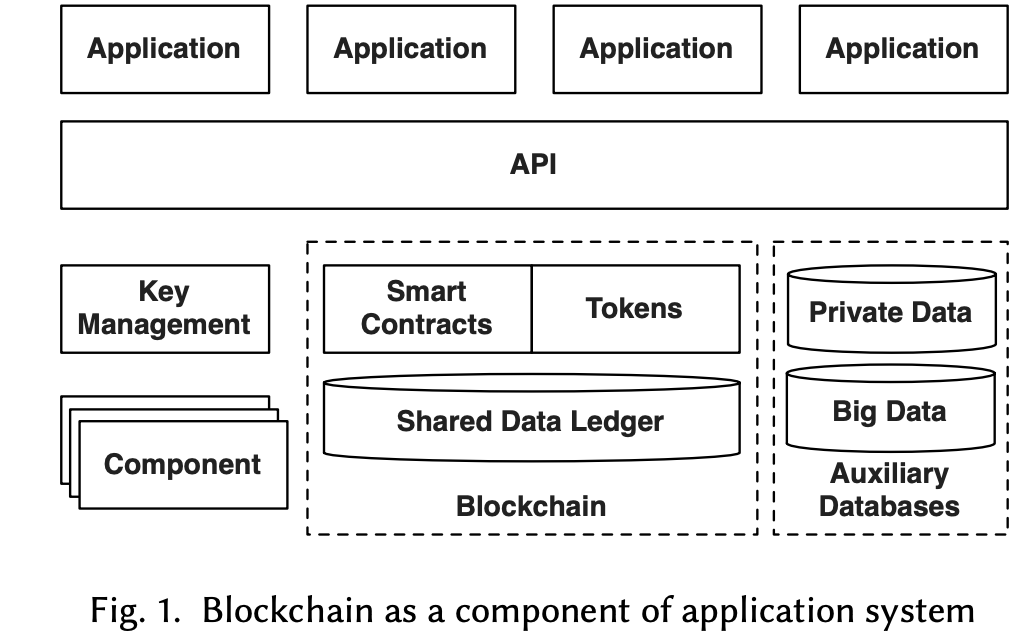
\includegraphics[width=0.9\textwidth]{images/architecture.png}}
    \caption{blockchain-based software application \label{fig:techstack} \cite{xuPatternCollectionBlockchainbased2018}}
\end{figure}

Due to its unique traits blockchain acts as a persistent, immutable and distributed data storage component in the overall architecture. As they are based on public-private key cryptography, there has to be a component, which is responsible for key management. Data which is too big, is stored in auxiliary databases and references are being stored on the blockchain. On top of the data storage layer, there is an API layer as seen in conventional applications. For the design of the prototype, a design process specified by Xu et al. has been used as an orientation. 

\textbf{Public or private ledger?}
Private Chains are not fully decentralized, whereas public chains have several challenges but can be tackled with. For a decentralized marketplace, it has to be assessed which property is more important. As described in the problem statement, a fully decentralized marketplace with no central authority and single point of failure has been defined as a requirement. Therefore fundamental properties will be the leading deciding factor.

The artefact should allow for anonymous payments and users also should be able to browse the marketplace without registering. 

Therefore a public and permission-less blockchain has been chosen. 

\textbf{data structure}
scalability, transaction costs, transaction time and network traffic and reliability has to be assessed. Blockchain offers the most trust which is needed in the application, thats why a blockchain has been decided upon. 

\textbf{on-chain or off-chain storage and computation?} 
In order to store value on the blockchain, each transaction is attached with a fee and therefore makes on-chain storage of data quite expensive.
The common way to circumvent this, is to store raw data off-chain and then to store the reference hash of the raw data on the blockchain since the amount of computational power and data storage space in the blockchain is limited. Off-chain data storage can be a private cloud/storage or public storage service provided by a third-party.  

 

%Author Xiui et al. proposes 4 common architectural patterns for integrating blockchain as part of the overall software system. Depending on the use case and requirements of a decentralized application, each pattern will have its advantages and disadvantages. Overall goal of applying those patterns is to decrease the impact of blockchain limitations and enhance its unique characteristics. According to the author, there do exist 4 different pattern types, which consist of external world patterns, contractual patterns, security pattern and data management pattern as can be seen in figure. 
% \cite[p. 52]{xuPatternCollectionBlockchainbased2018}


% \subsubsection {Motivation Blockchain Usage}
%Blockchain offer great capabilities for decentralized access control and registry services achieved through decentralized consensus and tamperproof storage of data and therefore will be used as backend of the artifact. 

\subsection{System Context}

In the domain of decentralized application marketplaces, there are the following actors: 

\subsubsection{Consumers}
The consumer party consists of one or more people, such as a private individual or employees of a company. They buy certain services, which are offered by service providers. 

\subsubsection{Service Provider}
Service provider can also be private individuals or companies. They sell their digital services to the consumer/costumer. 

\subsubsection{Identity Validators}
Independent organizations, who are allowed to issue verifiable identity claims. 

\subsubsection{App Validators}
independent organizations, who are allowed to issue verifiable claims about app quality. 

\subsection{Overview}
The blockchain-based application is implemented on top of the decentralized infrastructure mentioned in the introduction, called Blade. The following figure provides an overview of the components which are briefly described. 

\begin{figure}[htbp]
    \centerline{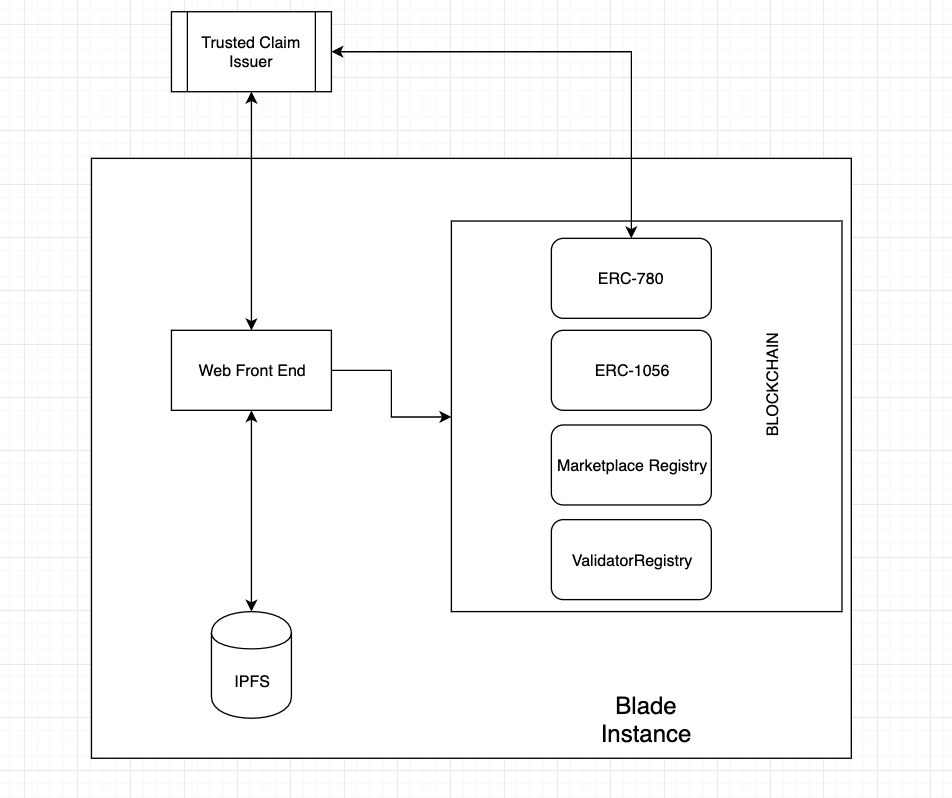
\includegraphics[width=0.9\textwidth]{figures/overview.png}}
    \caption{Architecture overview \label{fig:techstack}}
\end{figure}

\begin{enumerate}
    \item \textbf{Blade instance:}
    a machine having a blade instance installed providing the user with different interfaces in order to use the decentralized infrastructure including identity management and a marketplace interface. 
  
    \item \textbf{web frontend:} The web front end is the GUI user interface which allows the users to use the functionalities of the decentralized marketplace. 
  
    \item \textbf{distributed data storage IPFS:} The client can store its marketplace-related claims publicly available to its marketplace users. The storage is distributed and therefore accessible by other users even when the client is offline.  
  
    \item \textbf{blockchain component} This component contains several smart contracts dealing with data storage and providing access control functionality as well as decentralized identity management and data verification services. 
    
    \item \textbf{Registry server} The registry server fetches the blockchain log events and stores entity data on a local server. This increases look up time and query time for marketplace related data. 
    The server queries the DIDAttributeChanged of all Identities 
  
    \item \textbf{trusted claim issuers} These are trusted identity and app validators who issue claims for apps registered in the marketplace. people who upload app will need to get their apps certified by these independent validators. Validators will get a token and if the marketplace grows the token grows in value. Other users can now also buy apps with that token, so there is an economy surrounding the whole marketplace. 
  
\end{enumerate}

\subsection{API} 

The most important REST endpoints of the Registry server will be described in the following. 

Entity related data is stored tamperproof on the blockchain and IPFS storage. While data reliability and integrity is being enhanced greatly by the use of blockchain, data queriablity is very slow. In order to enhance this performance, a registry server will synchronize the data and store it in a local database such as e.g. mongodb, which offers sophisticated and fast query methods. 

\textbf{apps}

\begin{figure}[htbp]
    \centerline{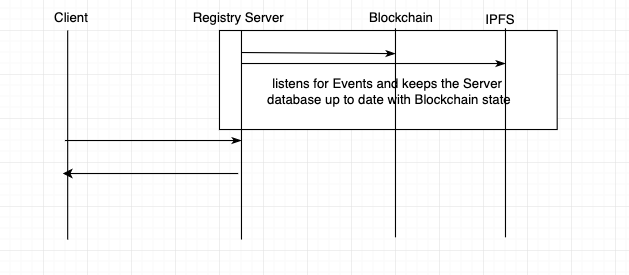
\includegraphics[width=0.9\textwidth]{figures/RegistryServer.png}}
    \caption{Fetching data \label{fig:registryServer}}
\end{figure}

\begin{table}[hbt!]
    \centering
    \caption{App}
    \begin{tabular}{llll}
    Method & Path      & Description         &   \\
    GET    & /apps     & get all Apps~       &   \\
    GET    & /apps/:id & get a specific app~ &   \\
           &           &                     &  
    \end{tabular}
\end{table}

\textbf{organizations} 

\textbf{apis}

\subsubsection{DIDResolver}

The DIDResolver builds upon the Ethr-DID-Resolver developed by uport, which enables ethereum addresses to be managed as decentralized identifiers compliant to the W3C specification. Every identity on the marketplace is represented through such a DID and its respective JSON document. The server uses this DID Resolver to resolve the decentralized IDs to their records. The DID Document for an app created in the marketplace looks like this: 

\begin{lstlisting}[caption={AppVersion}, language=Solidity, label=lst:appVersionFormat, numbers=none]
    {
      "@context": "https://w3id.org/did/v1",
      "id": "did:uport:2nQtiQG6Cgm1GYTBaaKAgr76uY7iSexUkqX",
      "publicKey": [{
        "id": "did:dmarket:2nQtiQG6Cgm1GYTBaaKAgr76uY7iSexUkqX#keys-1",
        "type": "Secp256k1VerificationKey2018",
        "owner": "did:dmarket:2nQtiQG6Cgm1GYTBaaKAgr76uY7iSexUkqX",
        "publicKeyHex": "04613bb3a4874d27032618f020614c21cbe4c4e4781687525f6674089f9bd3d6c7f6eb13569053d31715a3ba32e0b791b97922af6387f087d6b5548c06944ab062"
      }],
      "authentication": [{
        "type": "Secp256k1SignatureAuthentication2018",
        "publicKey": "did:dmarket:2nQtiQG6Cgm1GYTBaaKAgr76uY7iSexUkqX#keys-1"
      }],
      "dMarket": {
        "@context":"http://schema.org",
        "@type":"AppVersion",
        "app":"did:dmarket:3234234234234234234234",
        "version":"2", 
        "description":"Uport Attestations",
        "image":{"@type":"ImageObject","name":"avatar","contentUrl":"/ipfs/QmSCnmXC91Arz2gj934Ce4DeR7d9fULWRepjzGMX6SSazB"}
        "binaryLink": {"@type":"URLObject"},
        "supportedAPI":[]
      }
    }
\end{lstlisting}


\section{Identity Management}

Each service, organization or user is represented as an identity. Identities are represented by their Ethereum addresses. With the ERC-1056, those addresses are fully compliant to the WC3 DID Specification, thus each identity can be resolved to their respective DID document. 
Following assumptions regarding identity claim issuers have been made: there are trusted identity issuers existent, who issue verifiable identity claims to their subjects. Also they register a hash of that claim on the claim registry ERC780, mapping it to the specific subject of claim. 

\subsection{Registration of users}

The following figure provides an overview about the request flow made, when registering a user for the marketplace. 

\begin{figure}[htbp]
    \centerline{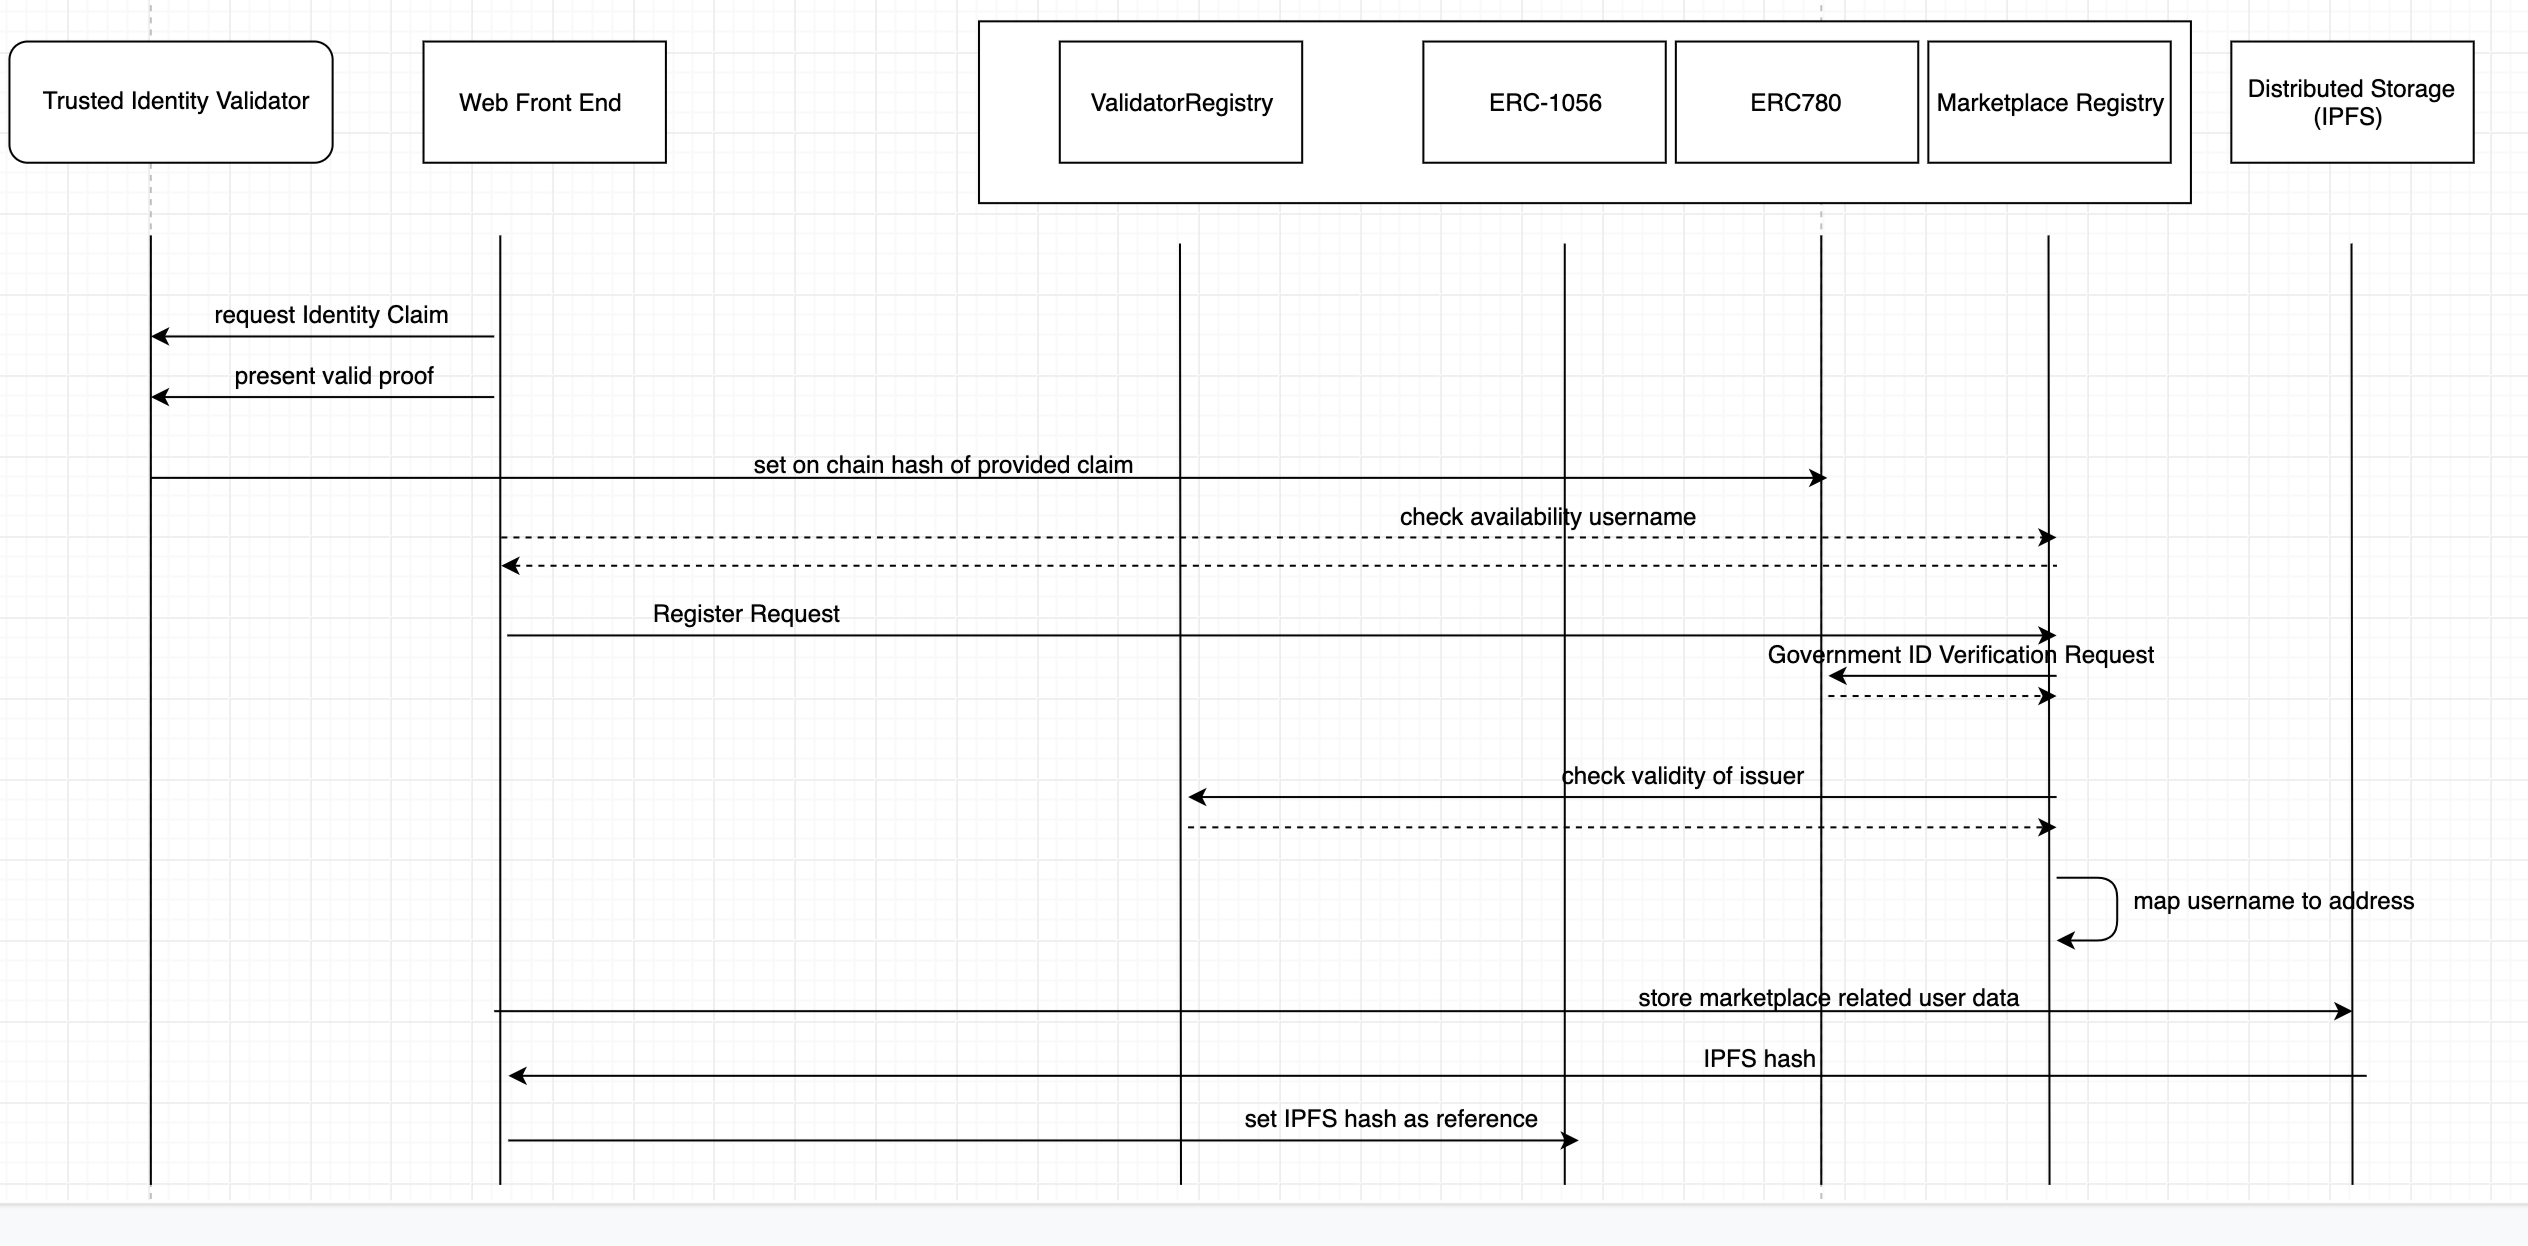
\includegraphics[width=0.9\textwidth]{figures/userRegistration.png}}
    \caption{Registration process \label{fig:registration}}
\end{figure}

Before registering on the marketplace, the user will be prompted to verify his identity at one of the accepted government ID validators. In this implementation, a stub validator will be implemented and we will assume that this entity is trustworthy. Once verified, the claim will be registered onchain. 

Now when registering a username, the marketplace registry will check for the government ID claim at the on-chain registry ERC-780 and if verification is successful, he will be able to register his username.

\subsection{Registration of Apps, Apis, Organizations}

Once a username is registered, he can register apps, api and organizations. Those will be called "entity" in the following. The registration consists of two steps: 
First, for each entity an Ethereum account will be created.
This public key will then be registered in the marketplace registry, which essentially acts as a name registry assigning human-friendly names on a first come, first served basis. 
When creating entities, the ownership over their DID documents will be transferred to the user, who created them. The registration of apps requires a marketplace specific claim verification schema, which has been showed in the data structures section. The marketplace registry has therefore a verification function, which will check wether the entity to be uploaded in IPFS conforms to that schema.

\section{Content Model}

Every User, App or Api, or Organization represents an identity and is being referenced by a unique decentralized identifier. This identifier follows the specification of a DID Document. Using decentralized identity fullfils the requirement of self souvereign data ownership. Each identity is being managed by its respective owner, and all data attached to that identity therefore belongs to them. 

% Every created entity is owned by its author. So in the normal case, the author is the same as the owner. But in case, that a user is creating a entity in the context of his organization, owner will be the organization. In either case, these roles are specified in the blockchain through cryptographic key management.  

\subsection{Related Work}

%{Decentralized Identifier} 

%{DID URL}

\subsection{Content Model}

This following content model conforms to the general DID specification. This data is being retrieved from the blockchain and will be presented as such by the DID resolver method. 

% THIS FUCKS UP THE FORMATTING. 
\begin{lstlisting}[caption={Example app content object}, language=Solidity, label=lst:content_model, numbers=none]
{
    "@context": "https://www.w3.org/ns/did/v1",
    "id": "did:example:123456789abcdefghi",
    "authentication": [{
        "id": "did:example:123456789abcdefghi#keys-1",
        "type": "RsaVerificationKey2018",
        "controller": "did:example:123456789abcdefghi",
        "publicKeyPem": "-----BEGIN PUBLIC KEY...END PUBLIC KEY-----"
    }],
    'dmarket': {
        '@context': 'http://schema.org',
        '@type': 'App',
        'name': 'Tawki',
        'owner': 'Microsoft',
        'author': "did:ethr:john"
        'description': 'Tawki is a decentralized chatting app making you feel very happy.',
        'image': {'@type': 'ImageObject', 'name': 'avatar', 'contentUrl': '/ipfs/QmSCnmXC91Arz2gj934Ce4DeR7d9fULWRepjzGMX6SSazB'},
        'versions': [{id:"...", type: "version", rating: "1.5"}, {id:"...", type: "version", rating: "2.5"}
    },
    "service": [{
        "id":"did:example:123456789abcdefghi#vcs",
        "type": "VerifiableCredentialService",
        "serviceEndpoint": "https://example.com/vc/"
    }]
}   
\end{lstlisting}


\subsection{Access Control Model}
% What is the goal of this model? User should be able to create organizations and assign control rights to added users. 

The goal of this model is to specify how access control can be handled with blockchain technology. If every organization or user could specify its own rules it actually would be optimal. Right now, role-based access control is being implemented. 

There is the possibility for app developers to create organizations and inviting multiple developers the organization. Therefore the attribute author specifies the person who created the entitiy (e.g. app or api), whereas owner specifies the ownership about the entity. For example, if Bob create an organization and invites Alices to the organization, he can choose to assign her one of those roles: Admin or Member. If Alice now creates an app within that organization, the app is owned by that organization but has been authored by Alice. If alice would leave the organization, then she would loose rights to edit this entity. 

\subsubsection{Roles} 
Those following roles do exist for the user. A user can be part of an organization and therefore gets a role assigned, if he joins an organization. Besides that, every user who creates an entity has the role of an author. Being the author usually means automatically being the owner as well, but not if he is part of an organization. 

\begin{enumerate}
    \item \textbf{Author:} The authorship authorizes the user to create, update or delete an entity.

    \item \textbf{Owner:} Being owner of an entity authorizes him/her to grant access to ressources of the marketplace. 

Within organizations: 

    \item \textbf{Admin:} The admin role authorizes the user to edit all entities within that organization. The admin has also the right to invite other users to the organization. 
    
    \item \textbf{Member:} being a member means to be able to create and edit their own entities within that organization. But they are not allowed to invite other members or edit the other entities besides their own. 
\end{enumerate}

\subsection{Service discovery}

% Registry Server Explanation

The DID Documents of registered entities will be resolved by a DID resolver. 
Since a public blockchain is being used, each transaction recorded is visible to everyone. The EIP712 proposal makes it possible to sign structured data to make verifiable off chain claims possible. For public apps or apis, the reference is stored on-chain as a DID attribute of their respective DID documents. This makes fetching the data more accessible. If the user would want to keep this data claims private, they could provide an endpoint from which other users could request this data. Another possibility would be to encrypt this data object with a secret via symmetric encryption and other users could request that secret in order to decrypt it. 



\subsection{Trust Mechanism}

\subsubsection{Sybil Attacks} 


\subsubsection{Service Quality}

This whole prototype is being designed with the idea of integrating decentralized identity in order to create trust while preserving the privacy of its users. In order to prevent sybil attacks and create trust in identity of app providers, users have to acquire a verifiable claim from the marketplace. The IdentityValidatorRegistry smart contract acts as a verifying instance. It will hold a list of trusted government ID validators and users will have to get their identity verified by these entities first. The marketplace will then authenticate user identity based on those claims, which will enable the users to interact on the service registry. 

Users who use that service registry can therefore be sure, that all provided apps are from real-world identities, without knowing any private information about those identities. 
Furthermore, to enhance trust in quality of apps, app validators could issue verifiable claims about the quality of those apps, too. 



\subsection{Verifiable Claims}
The DID Document is fetched  from the authenticator. It is fetched from a Verifiable Data Registry! The  Verifiable Data Registry holds all Deentralized Identities and their Keys. 

The authenticator/ verifier can verify all signed data by that registry. 

Because the registry holds the data schema for that OFF chain data, and the identifier/key used in conjunction with the issuer of the data is registered. One can verify that this data is conforming to that schema and has been signed by that authority. 

The schema is important because it defines the structure of the claim, and also an explanation of the claim, what validators can expect from it. 


Now the problem is my marketplace is a smart contract. It does not have authentication keys. It doesn'T sign messages with a signature. 

A way to solve this is with an onchain Claim. 

We don't resolve the DID document of marketplace and check for the signature, but we ask ERC780 for validation. 

Now the cool thing about verifiable Claims is, that the claim itself is a readable JSON in the structure already. It can be nested and complex as fuck, it doesnt matter since only the signature of it matters. And because the signature is deeply coupled with the content, once I use that signature and that hash and it returns me the public key , i Know it has not been altered and I know yeah, that claim is valid. The subject know just has to proof that he is the subject and then it is alright. 

Now because the smart contract cannot sign that verifiable Claim, I will just let the subject sign that shit! 

This will generate me a signature. 

Issuer  : Marketplace 
Subject: Subject Address
Data : Hash  / Claim ID, Claim Key  

Verification 

Take Data verify its schema -> Check. 
Signature is not needed, because the client will have to check that issuer in the claim indeed is the issuer address set in ERC780. 

Now hash that claim with 
\chapter{Implementation}
\label{cha:implementation}

In this chapter the construction of a prototype will be described. 
This section will give an overview about the actual implementation details. It shall enable the user to use and configure the prototype. First, the overall structure of the codebase will be explained. Then, more details about the actual implementation of the smart contracts are described. The marketplace interface is explained at last. 

\section{codebase}

\section{Structure of Smart Contracts}

An overview of the smart contracts is shown in Figure 4. Various functionalities of the prototype has been split into different contracts and  inheritance was being used as a means to combine them meaningfully. 
 
Because Identity Management is becoming more and more of an issue, my prototype wants to enable self souvereign identity. 
This means, that users should have full control over their data and their privacy settings. A public private key pair already represents an identity. To conform to the W3C standard, that key has to be referenced with certain data. 

ERC1056 has been chosen, because it offers decentralized management of identifiers. 


\chapter{Evaluation}
\label{cha:evaluation}

[Version 1]
In the following chapter, the last step of the DSRM process will be executed.  First, a literature review is conducted in order to identify challenges towards centralized and decentralized application marketplaces. Then, the developed prototype will be evaluated against the necessary requirements derived from these identified challenges. At last, a quantitative evaluation of the prototype's performance is shown. 

General challenges towards digital marketplaces - centralized as well as decentralized - is the creation of trust among the users. 

Centralized platforms use reputation systems in order to create this trust and charge buyers and sellers a horrendous amount. Ich brauch Quellen !! 
 
\chapter{Conclusion}
\label{cha:conclusion}

Describe what you did here

%--------------------------------------------------------------
% TABLES, FIGURES, BIBLOGRAPHY AND APPENDICES
%--------------------------------------------------------------
\backmatter

% Lists of tables and figures
\listoftables
\listoffigures

% Bibliography
\setwidesite{}						% Set page to be wider for bibliography
\markboth{Bibliography}{bibliography}
\label{cha:bibliography}
\bibliographystyle{IEEEtran}
\bibliography{end.bib}

% Use following to separate online (websites) and offline (books, papers) sources
%\printbibliography[heading=offline,filter=offline]
%\printbibliography[heading=online,filter=online]

\begin{appendices}
	\chapter{Appendix 1}
\label{appendix:listing1}

\lstset{language=PHP}
\begin{lstlisting}
for($i=1; $i<123; $i++)
{
    echo "work harder! ;)";
}
\end{lstlisting}
	% \input{content/99_appendices/a02_listings}
	% \input{content/99_appendices/a03_listings}
\end{appendices}

\end{document}
